\documentclass{standalone}
\usepackage{tikz}
\usetikzlibrary{patterns, positioning}
\usepackage[sfdefault]{ClearSans} %% option 'sfdefault' activates Clear Sans as the default text font
\usepackage[T1]{fontenc}

\begin{document}
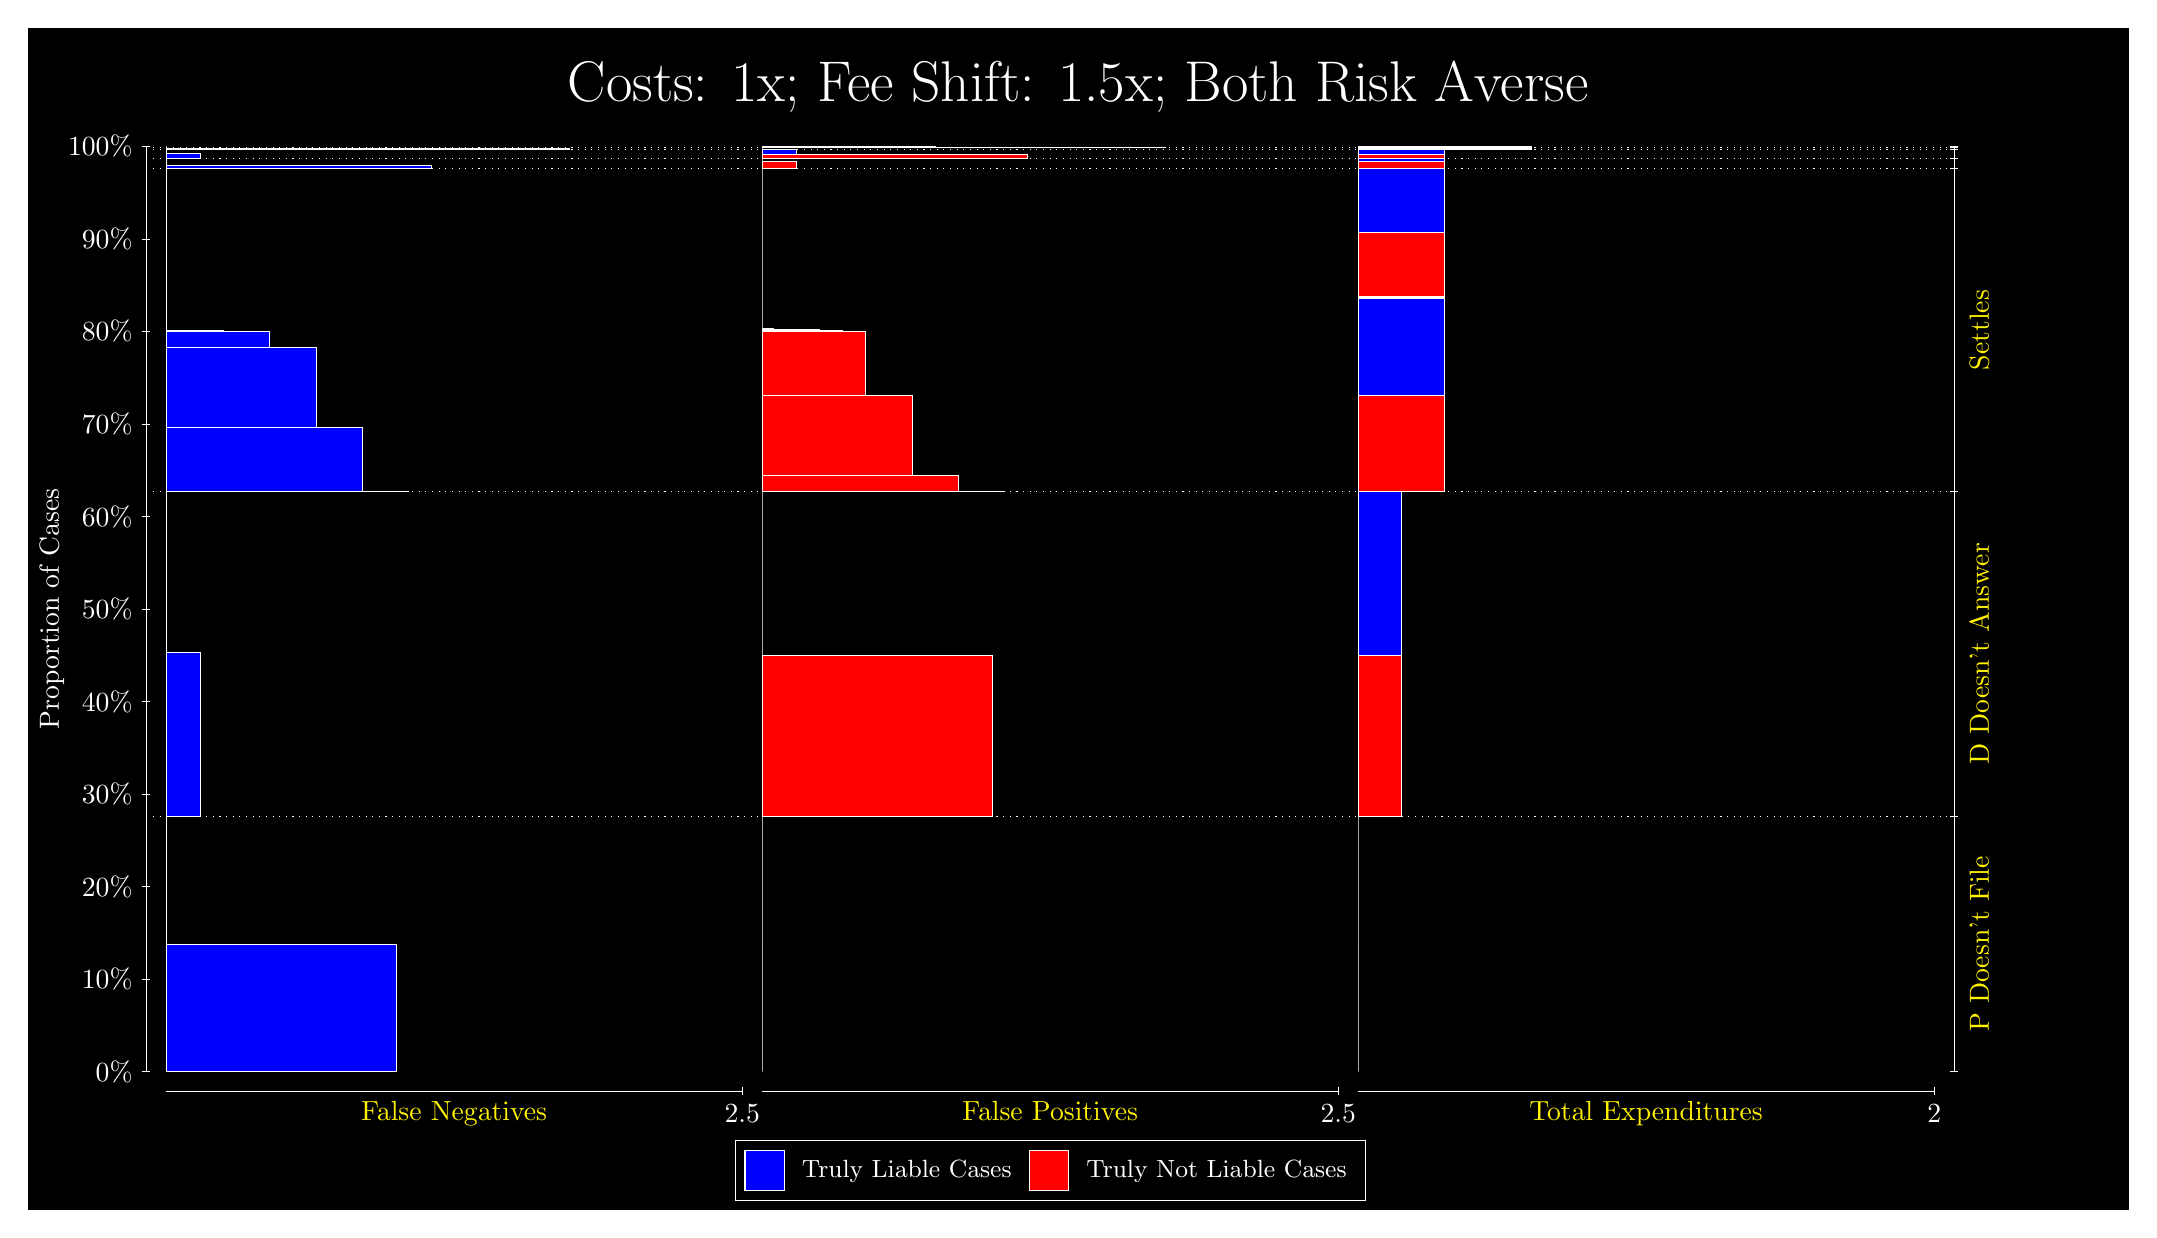
\begin{tikzpicture}
\draw[fill=black] (0,0) rectangle (26.667,15);
\draw[text=white] (0,13.5) rectangle (26.667,15) node[midway] {\huge Costs: 1x; Fee Shift: 1.5x; Both Risk Averse};
\draw[white, very thin] (1.5,1.75) -- (1.5,13.5);
\node[rotate=90, text=white, anchor=center] at (0.3, 7.625) {Proportion of Cases};
\draw[white, very thin] (1.45,1.75) -- (1.55,1.75);
\node[text=white, anchor=east] at (1.45, 1.75) {0\%};
\draw[white, very thin] (1.45,2.925) -- (1.55,2.925);
\node[text=white, anchor=east] at (1.45, 2.925) {10\%};
\draw[white, very thin] (1.45,4.1) -- (1.55,4.1);
\node[text=white, anchor=east] at (1.45, 4.1) {20\%};
\draw[white, very thin] (1.45,5.275) -- (1.55,5.275);
\node[text=white, anchor=east] at (1.45, 5.275) {30\%};
\draw[white, very thin] (1.45,6.45) -- (1.55,6.45);
\node[text=white, anchor=east] at (1.45, 6.45) {40\%};
\draw[white, very thin] (1.45,7.625) -- (1.55,7.625);
\node[text=white, anchor=east] at (1.45, 7.625) {50\%};
\draw[white, very thin] (1.45,8.8) -- (1.55,8.8);
\node[text=white, anchor=east] at (1.45, 8.8) {60\%};
\draw[white, very thin] (1.45,9.975) -- (1.55,9.975);
\node[text=white, anchor=east] at (1.45, 9.975) {70\%};
\draw[white, very thin] (1.45,11.15) -- (1.55,11.15);
\node[text=white, anchor=east] at (1.45, 11.15) {80\%};
\draw[white, very thin] (1.45,12.325) -- (1.55,12.325);
\node[text=white, anchor=east] at (1.45, 12.325) {90\%};
\draw[white, very thin] (1.45,13.5) -- (1.55,13.5);
\node[text=white, anchor=east] at (1.45, 13.5) {100\%};

\draw[white, very thin] (24.457,1.75) -- (24.457,13.5);
\draw[white, very thin] (24.407,1.75) -- (24.507,1.75);
\node[anchor=west] at (24.407, 1.75) {};
\draw[white, very thin] (24.407,4.9914) -- (24.507,4.9914);
\node[anchor=west] at (24.407, 4.9914) {};
\draw[white, very thin] (24.407,9.1139) -- (24.507,9.1139);
\node[anchor=west] at (24.407, 9.1139) {};
\draw[white, very thin] (24.407,13.223) -- (24.507,13.223);
\node[anchor=west] at (24.407, 13.223) {};
\draw[white, very thin] (24.407,13.344) -- (24.507,13.344);
\node[anchor=west] at (24.407, 13.344) {};
\draw[white, very thin] (24.407,13.464) -- (24.507,13.464);
\node[anchor=west] at (24.407, 13.464) {};
\draw[white, very thin] (24.407,13.482) -- (24.507,13.482);
\node[anchor=west] at (24.407, 13.482) {};
\draw[white, very thin] (24.407,13.5) -- (24.507,13.5);
\node[anchor=west] at (24.407, 13.5) {};

\draw[white, very thin, fill=blue] (1.75,1.75) rectangle (4.6775,3.3707);
\draw[white, very thin, fill=red] (1.75,3.3707) rectangle (1.75,4.9914);
\draw[white, very thin, fill=blue] (1.75,4.9914) rectangle (2.1891,7.0686);
\draw[white, very thin, fill=red] (1.75,7.0686) rectangle (1.75,9.1139);
\draw[white, very thin, fill=blue] (1.75,9.1139) rectangle (4.8239,9.1168);
\draw[white, very thin, fill=blue] (1.75,9.1168) rectangle (4.5312,9.1201);
\draw[white, very thin, fill=blue] (1.75,9.1201) rectangle (4.2384,9.9308);
\draw[white, very thin, fill=blue] (1.75,9.9308) rectangle (3.9457,9.9309);
\draw[white, very thin, fill=blue] (1.75,9.9309) rectangle (3.6529,10.945);
\draw[white, very thin, fill=blue] (1.75,10.945) rectangle (3.3602,10.945);
\draw[white, very thin, fill=blue] (1.75,10.945) rectangle (3.0674,11.148);
\draw[white, very thin, fill=blue] (1.75,11.148) rectangle (2.7746,11.153);
\draw[white, very thin, fill=blue] (1.75,11.153) rectangle (2.4819,11.165);
\draw[white, very thin, fill=red] (1.75,11.165) rectangle (1.75,13.223);
\draw[white, very thin, fill=blue] (1.75,13.223) rectangle (5.1167,13.262);
\draw[white, very thin, fill=red] (1.75,13.262) rectangle (1.75,13.344);
\draw[white, very thin, fill=blue] (1.75,13.344) rectangle (2.1891,13.413);
\draw[white, very thin, fill=red] (1.75,13.413) rectangle (1.75,13.464);
\draw[white, very thin, fill=blue] (1.75,13.464) rectangle (6.8732,13.471);
\draw[white, very thin, fill=red] (1.75,13.471) rectangle (1.75,13.482);
\draw[white, very thin, fill=red] (1.75,13.482) rectangle (1.75,13.489);
\draw[white, very thin, fill=blue] (1.75,13.489) rectangle (1.75,13.5);
\draw[white, very thin, fill=red] (9.3189,1.75) rectangle (9.3189,3.3707);
\draw[white, very thin, fill=blue] (9.3189,3.3707) rectangle (9.3189,4.9914);
\draw[white, very thin, fill=red] (9.3189,4.9914) rectangle (12.246,7.0367);
\draw[white, very thin, fill=blue] (9.3189,7.0367) rectangle (9.3189,9.1139);
\draw[white, very thin, fill=red] (9.3189,9.1139) rectangle (12.393,9.1183);
\draw[white, very thin, fill=red] (9.3189,9.1183) rectangle (12.1,9.1234);
\draw[white, very thin, fill=red] (9.3189,9.1234) rectangle (11.807,9.3265);
\draw[white, very thin, fill=red] (9.3189,9.3265) rectangle (11.515,9.3267);
\draw[white, very thin, fill=red] (9.3189,9.3267) rectangle (11.222,10.341);
\draw[white, very thin, fill=red] (9.3189,10.341) rectangle (10.929,10.341);
\draw[white, very thin, fill=red] (9.3189,10.341) rectangle (10.636,11.152);
\draw[white, very thin, fill=red] (9.3189,11.152) rectangle (10.344,11.159);
\draw[white, very thin, fill=red] (9.3189,11.159) rectangle (10.051,11.172);
\draw[white, very thin, fill=blue] (9.3189,11.172) rectangle (9.4652,11.183);
\draw[white, very thin, fill=blue] (9.3189,11.183) rectangle (9.3189,13.223);
\draw[white, very thin, fill=red] (9.3189,13.223) rectangle (9.758,13.304);
\draw[white, very thin, fill=blue] (9.3189,13.304) rectangle (9.3189,13.344);
\draw[white, very thin, fill=red] (9.3189,13.344) rectangle (12.686,13.395);
\draw[white, very thin, fill=blue] (9.3189,13.395) rectangle (9.758,13.464);
\draw[white, very thin, fill=red] (9.3189,13.464) rectangle (9.3189,13.476);
\draw[white, very thin, fill=blue] (9.3189,13.476) rectangle (9.3189,13.482);
\draw[white, very thin, fill=red] (9.3189,13.482) rectangle (14.442,13.489);
\draw[white, very thin, fill=blue] (9.3189,13.489) rectangle (11.515,13.5);
\draw[white, very thin, fill=red] (16.888,1.75) rectangle (16.888,3.3707);
\draw[white, very thin, fill=blue] (16.888,3.3707) rectangle (16.888,4.9914);
\draw[white, very thin, fill=red] (16.888,4.9914) rectangle (17.437,7.0367);
\draw[white, very thin, fill=blue] (16.888,7.0367) rectangle (17.437,9.1139);
\draw[white, very thin, fill=red] (16.888,9.1139) rectangle (17.986,10.341);
\draw[white, very thin, fill=blue] (16.888,10.341) rectangle (17.986,11.574);
\draw[white, very thin, fill=red] (16.888,11.574) rectangle (17.986,11.587);
\draw[white, very thin, fill=blue] (16.888,11.587) rectangle (17.986,11.59);
\draw[white, very thin, fill=red] (16.888,11.59) rectangle (17.986,12.408);
\draw[white, very thin, fill=blue] (16.888,12.408) rectangle (17.986,13.223);
\draw[white, very thin, fill=red] (16.888,13.223) rectangle (17.986,13.304);
\draw[white, very thin, fill=blue] (16.888,13.304) rectangle (17.986,13.344);
\draw[white, very thin, fill=red] (16.888,13.344) rectangle (17.986,13.395);
\draw[white, very thin, fill=blue] (16.888,13.395) rectangle (17.986,13.464);
\draw[white, very thin, fill=red] (16.888,13.464) rectangle (19.083,13.476);
\draw[white, very thin, fill=blue] (16.888,13.476) rectangle (19.083,13.482);
\draw[white, very thin, fill=red] (16.888,13.482) rectangle (19.083,13.489);
\draw[white, very thin, fill=blue] (16.888,13.489) rectangle (19.083,13.5);
\draw[white, dotted] (1.5,4.9914) -- (24.457,4.9914);
\draw[white, dotted] (1.5,9.1139) -- (24.457,9.1139);
\draw[white, dotted] (1.5,13.223) -- (24.457,13.223);
\draw[white, dotted] (1.5,13.344) -- (24.457,13.344);
\draw[white, dotted] (1.5,13.464) -- (24.457,13.464);
\draw[white, dotted] (1.5,13.482) -- (24.457,13.482);
\draw[white, very thin] (1.75,1.5) -- (9.0689,1.5);
\node[text=yellow, anchor=north] at (5.4094, 1.5) {False Negatives};
\draw[white, very thin] (9.0689,1.45) -- (9.0689,1.55);
\node[text=white, anchor=north] at (9.0689, 1.45) {2.5};

\draw[white, very thin] (9.3189,1.5) -- (16.638,1.5);
\node[text=yellow, anchor=north] at (12.978, 1.5) {False Positives};
\draw[white, very thin] (16.638,1.45) -- (16.638,1.55);
\node[text=white, anchor=north] at (16.638, 1.45) {2.5};

\draw[white, very thin] (16.888,1.5) -- (24.207,1.5);
\node[text=yellow, anchor=north] at (20.547, 1.5) {Total Expenditures};
\draw[white, very thin] (24.207,1.45) -- (24.207,1.55);
\node[text=white, anchor=north] at (24.207, 1.45) {2};

\node[text=yellow, centered, rotate=90] at (24.777, 3.3707) {P Doesn't File};
\node[text=yellow, centered, rotate=90] at (24.777, 7.0527) {D Doesn't Answer};
\node[text=yellow, centered, rotate=90] at (24.777, 11.168) {Settles};





\draw (12.978300999999998,1.5) node[draw=none] (baseCoordinate) {};
\begin{scope}[align=center]
        \matrix[scale=0.5, draw=white, below=0.5cm of baseCoordinate, nodes={draw}, column sep=0.1cm]{
            \node[rectangle, draw, minimum width=0.5cm, minimum height=0.5cm, fill=blue] {}; &
            \node[draw=none, font=\small, text=white] (B) {Truly Liable Cases}; &
            \node[rectangle, draw, minimum width=0.5cm, minimum height=0.5cm, fill=red] {}; &
            \node[draw=none, font=\small, text=white] (B) {Truly Not Liable Cases}; \\
            };
\end{scope}

\end{tikzpicture}
\end{document}